\documentclass[UTF8]{ctexart}
\usepackage{graphicx}
\usepackage{float}
\usepackage{geometry}
\usepackage{fancyhdr}
\usepackage{lastpage}
\usepackage{subfigure}
\geometry{left=2.54cm,right=2.54cm,top=3.18cm,bottom=3.18cm}%页边距
\pagestyle{fancy}
\lhead{\includegraphics[scale=1]{sjtu-logo-red.pdf}}  
\rhead{Intel与AMD处理器发展历程报告} 
\cfoot{第 \thepage\ 页\ 共 \pageref{LastPage} 页} 

\begin{document}

\begin{titlepage}
    \begin{center}
        \includegraphics[width=0.8\textwidth]{sjtu-name-blue.pdf}\\[1cm]
        \textsc{\Huge \bfseries 课程报告}\\[1.5cm]
        \includegraphics[width=0.3\textwidth]{sjtu-badge-blue.pdf}\\[0.5cm]

        \Huge \bfseries{Intel与AMD处理器发展历程报告}\\[1cm]
        \Large \bfseries{518021910971 裴奕博}
    \end{center}
\end{titlepage}
\section{CPU发展概述}
1947年12月,由美国贝尔实验室的肖克利、巴丁和布拉顿组成的研究小组,发明了晶体管。这种新的材料工艺相比之前的真空电子管,体积小巧、无需预热、耗能极低,很快取代了电子管成为了新一代电子电路的首选。在随后的几十年间,伴随着集成电路的发明,由这种材料制成的电子电路规模越来越大。从小规模、中规模集成电路到大规模、超大规模集成电路。

随着人类对计算机计算能力和便携性的要求不断提升,人们提出了“微型计算机”的概念,要实现这一点,首当其冲的就是将计算机的中央处理单元小型化。1971年,Intel公司制造出了第一个商用微处理器即4004,也宣告了第四代计算机时代的来临。从1971年至今的近50年间,随着个人计算机(PC)的成熟、发展和普及,作为计算机核心的CPU也得以迅猛发展。两家“本是同根生”的半导体公司,Intel和AMD,在这几十年间共同促成了CPU技术的不断提升,时至今日也是市面上处理器的最主流选择。本报告即梳理了从1971年至今,两家公司系列处理器的发展历程。
\section{Intel系列处理器发展历程}

\subsection{1968-1978 Intel公司的创立与4004处理器的诞生}
\subsubsection{Intel的创立}
1955年,晶体管的发明者威廉·肖克利离开贝尔实验室,创建了肖克利半导体实验室,并且吸引了一大批有才华的年轻科学家加入。但很快,由于内部原因,其中8名科学家联合辞职创办了仙童半导体公司,其中就包括摩尔定律的提出者戈登·摩尔(Gordon Moore)和集成电路的联合发明人罗伯特·诺伊斯(Robert Noyce)。1968年,两人从仙童半导体公司辞职,在7月16日共同创办Intel公司。其名称来源于集成电路(Integrated Electronics)的首字母缩写。
\begin{figure}[H]
    \begin{center}
        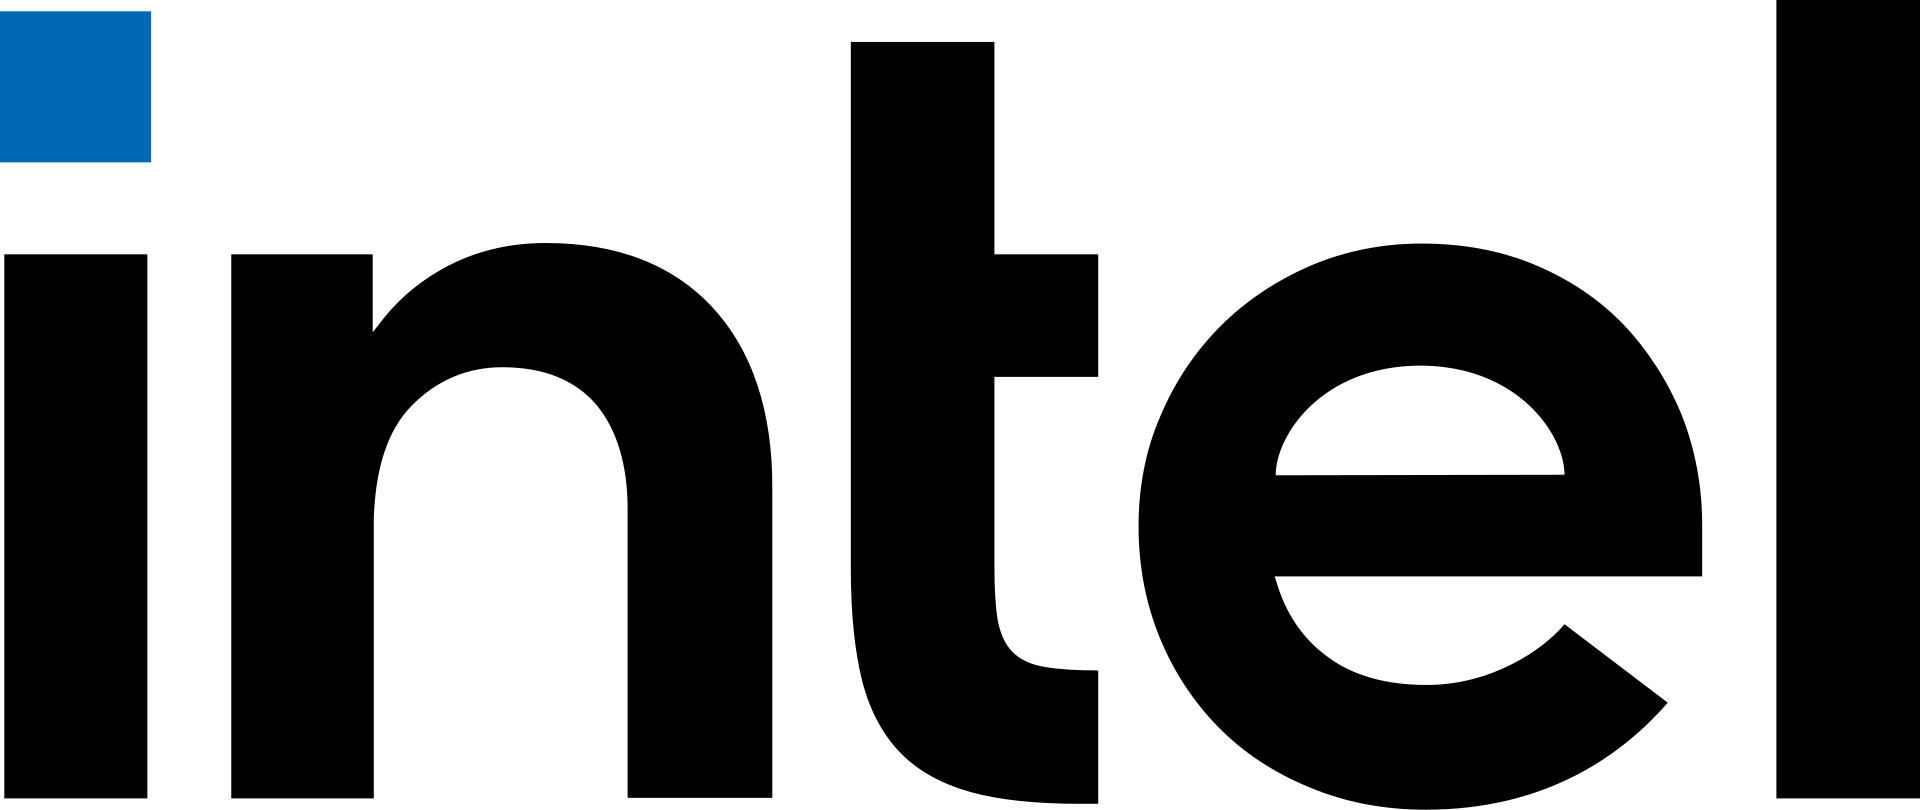
\includegraphics[width=0.2\textwidth]{figure/intel.png}
        \caption{Intel公司现在的logo}
    \end{center}
\end{figure}
起初,Intel的业务主要来自半导体存储器市场,主攻DARM和SARM,在整个20世纪70年代,CPU都不是Intel最主要业务。1971年11月15日,Intel的工程师霍夫(Marcian Hoff)发明了世界上第一块大规模集成电路,也是第一颗微处理器Intel 4004。恐怕那时Intel公司自己也未曾想到,这一天将被永远载入史册,这一“无心之举”也成为了Intel在今后几十年绝大部分的收入来源。

\subsubsection{Intel 4004}
4004处理器起初只是用于在日本Busicom公司生产的计算器中替换一些应用导向集成电路。它只有4位,45条指令,最高主频也仅有740kHz,甚至比不上ENIAC。但由于它集成化程度高,体积小,为个人计算机的发展铺平了道路,具有重要的里程碑意义。
\begin{figure}[H]
    \begin{center}
        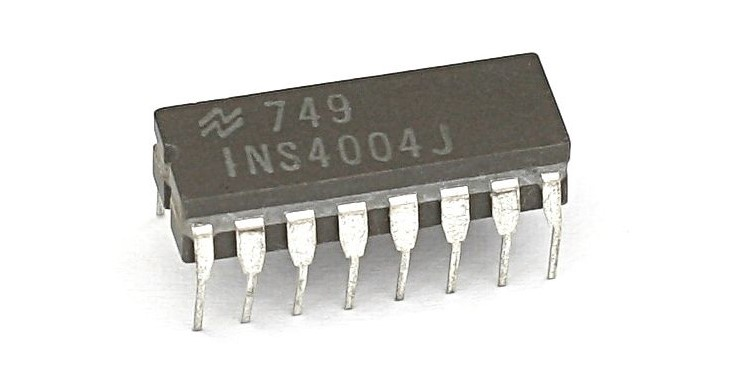
\includegraphics[width=0.4\textwidth]{figure/4004.jpg}
        \caption{Intel 4004}
    \end{center}
\end{figure}

\subsubsection{Intel 8008/8080}
在接下来的几年中,Intel又推出了8位的8008(1972)和8080(1974)处理器。在研发8008的过程中,Intel还获得了由德州的Datapoint公司开发的指令集,正是这套指令集,奠定了今天x86系列指令集的基础。与此同时,微处理器的优势也逐渐被人们所认同。尤其是8080处理器获得了空前的成功。该处理器主频为2MHz,性能是8008的十倍。作为人类历史上的第一台个人计算机Altair也使用了8080处理器作为核心。
\begin{figure}[H]
    \centering
    \subfigure[Intel 8008]{
        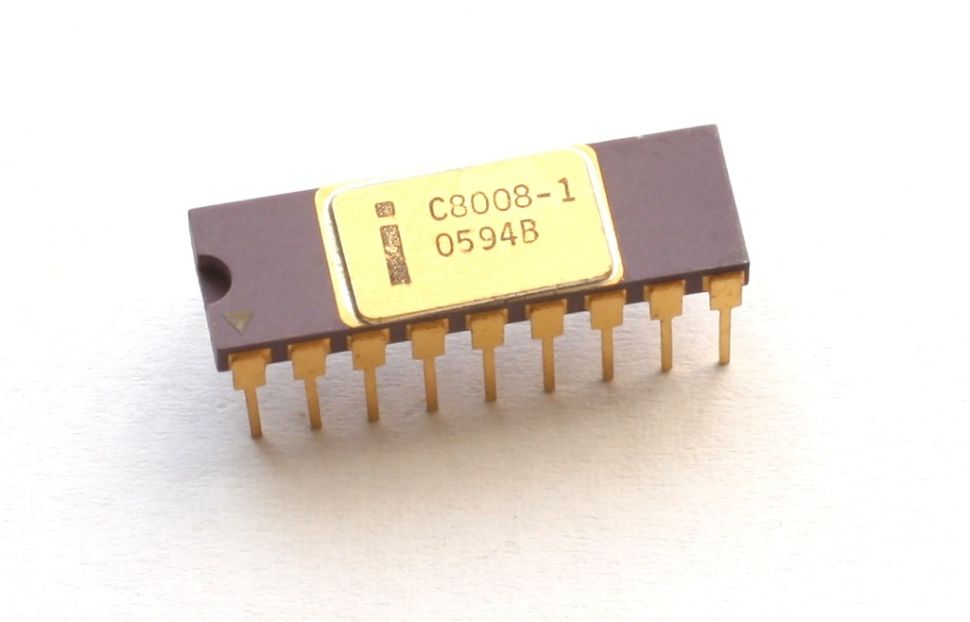
\includegraphics[width=0.5\textwidth]{figure/8008.jpg}
    }
    \subfigure[Intel 8080]{
        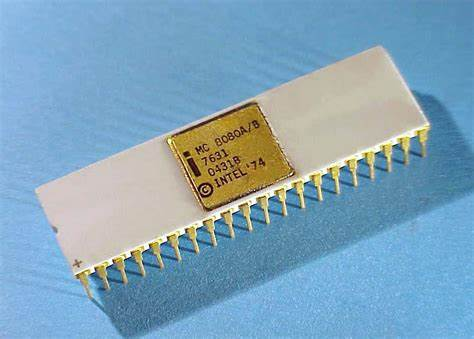
\includegraphics[width=0.4\textwidth]{figure/8080.jpg}
    }
    \caption{Intel 8008/8080}
\end{figure}

\subsection{1978-1993 x86系列处理器与x86指令集的开端}
这一阶段,Intel以8086处理器为开端,开创了x86指令集架构,这一架构也对未来的处理器发展有着深远影响。
\subsubsection{Intel 8086/8088}
1978年,Intel推出了8086处理器。它有16位的数据总线,可一次读取1MB内存,是Intel推出的首个16位处理器。与此同时,Intel还在其上使用了x86指令集。子从那时起,几乎所有的Intel和AMD处理器的指令集都是基于该指令集。从此,x86也成为了个人计算机的标准平台,也是历来最成功的CPU架构之一。

几乎与此同时,Intel也推出了8088处理器,将地址总线提升至20bit。两款处理器都采用了相同的16位x86架构。
\begin{figure}[H]
    \begin{center}
        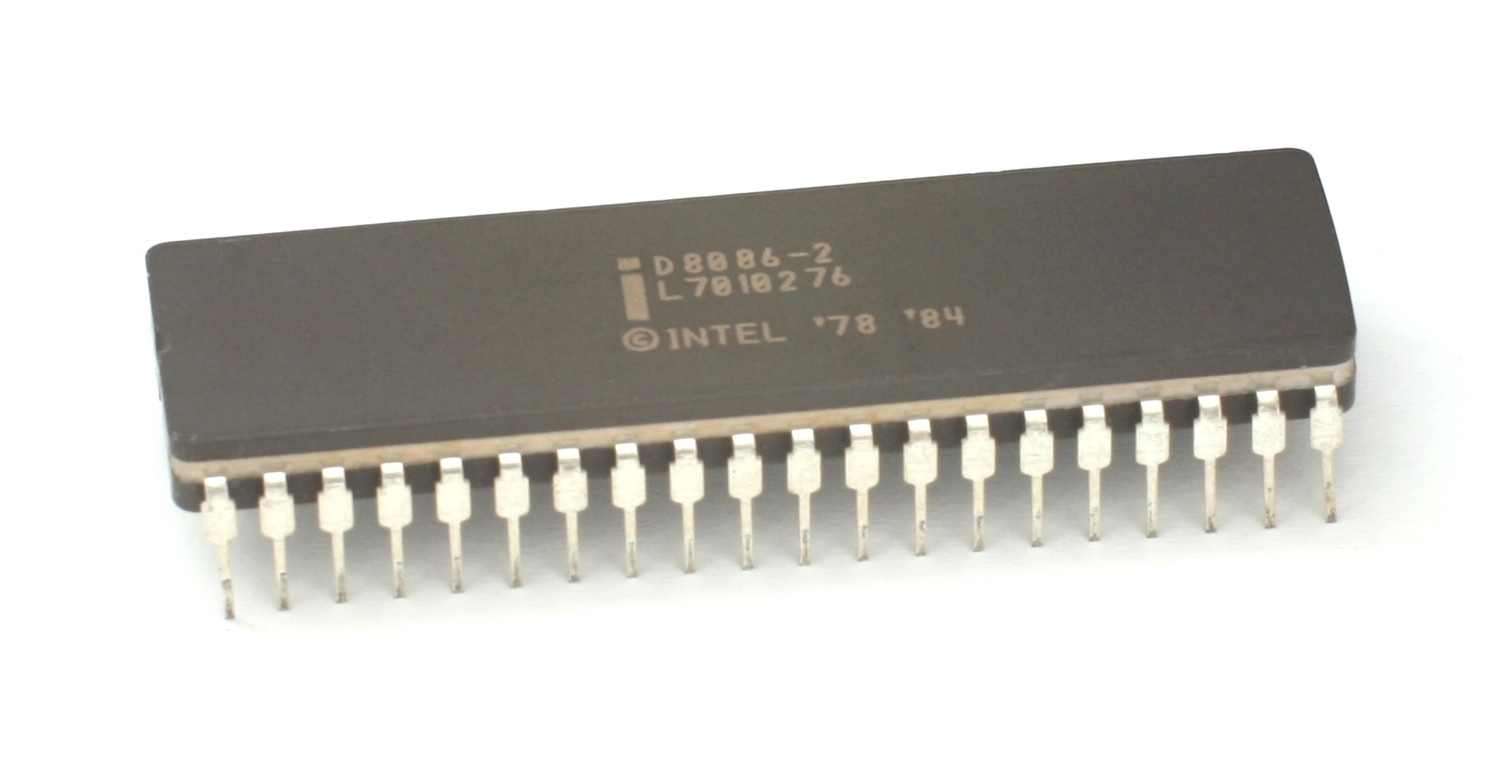
\includegraphics[width=0.4\textwidth]{figure/8086.jpg}
        \caption{Intel 8086}
    \end{center}
\end{figure}

\subsubsection{Intel 80x86系列}
随着PC市场需求的一步步扩大,CPU业务逐渐成为了Intel的主业。从1980年起,Intel接连推出了一系列基于x86架构的处理器,包括80186(1980)、80188(1980)、80286(1982)、80386(1985)和80486(1989)。
\begin{figure}[H]
    \centering
    \subfigure[Intel 80186]{
        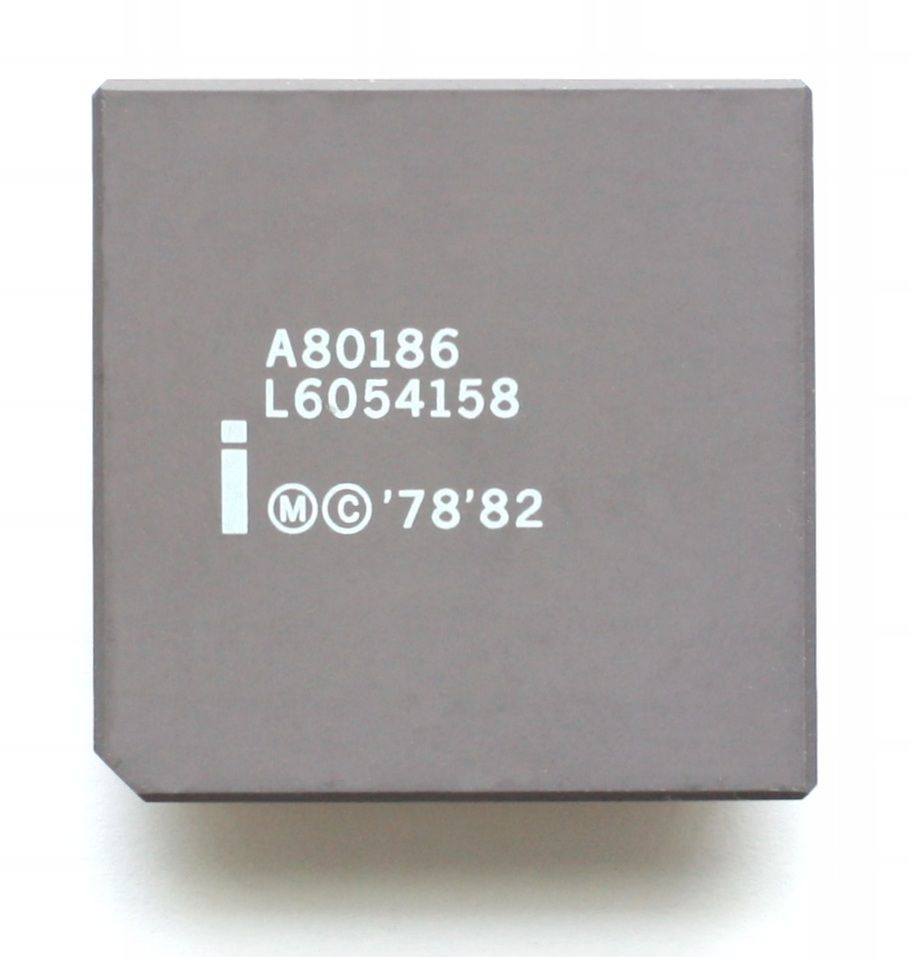
\includegraphics[width=0.3\textwidth]{figure/80186.jpg}
    }
    \subfigure[Intel 80486]{
        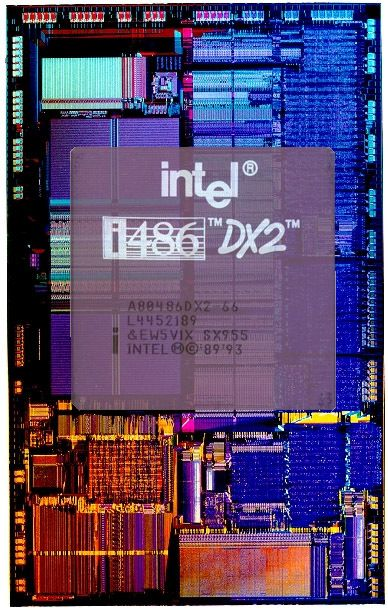
\includegraphics[width=0.2\textwidth]{figure/80486.jpg}
    }
    \caption{Intel 80186和80486}
\end{figure}
其中,80188和80186几乎同时推出,80188削减了一半的外部数据总线以降低成本。80286是Intel第一款完全兼容前代CPU的处理器。

从1985年的80386开始,Intel系列处理器进入32位时代,32位的x86架构也称为IA-32。80386集成了27万多只晶体管,规模超过了了初代CPU 4004的100倍,同时也是第一款具有多任务功能的处理器,这也为操作系统的发展有重要影响。

1989年,Intel发布了最后一款用数字命名的处理器——Intel 80486。在这一代CPU上,Intel首次将FPU(浮点计算单元)集成在CPU之内。此外,8KB的L1缓存第一次出现在了x86 CPU上。


\subsection{1993-2006 奔腾(Pentium)时代}
经过一系列80x86处理器,Intel已经从一家主攻存储芯片的公司,转为CPU领域的霸主。1993年,Intel发布了以子商标奔腾(Pentium)命名的处理器,正式宣告处理器进入奔腾时代。
\subsubsection{Pentium与Pentium MMX}
1993年,采用P5架构的Pentium处理器发布,而没有遵循80x86号码系统。这是一个划时代的事件。在接下来的十几年间,奔腾几乎成为了家喻户晓的名字,时至今日仍在使用。初代Pentium系列将CPU的工作电压降至3.3V,增强了浮点数的运算,新使用的P5架构使得它在所有方面都比80486快。1994年,Pentium处理器被发现在浮点数的计算上出现了瑕疵,Intel不得不召回大批的Pentium处理器。

然而这一事件并未影响Intel在CPU领域的高歌猛进。1996年,主攻服务器方向,采用P6架构的Pentium Pro推出。1997年1月,Pentium MMX推出。它扩展了L1缓存至16KB,也扩展了新的MMX指令集,使得其对多媒体数据的处理更为强大,也因此红极一时。此外,MMX系列的处理器还拥有较强的超频能力,还能通过提高其核心电压来获得更好的性能。1997年,同样采用P6架构的Pentium \uppercase\expandafter{\romannumeral2}发布,L1缓存已经增加到16KB数据缓存+16KB指令缓存共32KB。
\begin{figure}[H]
    \centering
    \subfigure[Pentium MMX]{
        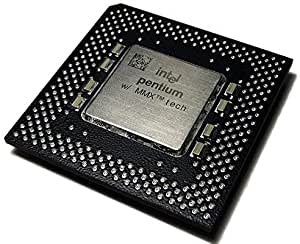
\includegraphics[width=0.25\textwidth]{figure/pentium.jpg}
    }
    \subfigure[Pentium Pro]{
        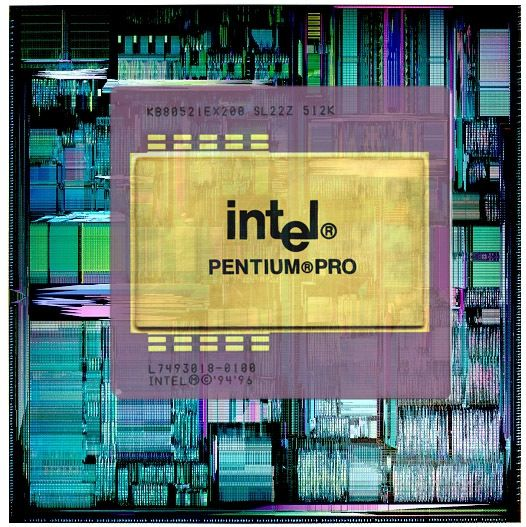
\includegraphics[width=0.2\textwidth]{figure/pentium_pro.jpg}
    }
    \caption{Pentium和Pentium Pro}
\end{figure}

\subsubsection{赛扬(Celeron)和至强(Xeon)}
1998年,随着AMD大举入侵低价处理器市场,而同期的Pentium \uppercase\expandafter{\romannumeral2}价格昂贵。为了兼顾低端市场,Intel将Pentium \uppercase\expandafter{\romannumeral2}中的两颗L2缓存取消,推出了初代Celeron处理器,从此诞生了“赛扬”这一新的产品线。

同时,为区分服务器市场与PC市场,英特尔还推出了Pentium \uppercase\expandafter{\romannumeral2} Xeon作为Pentium Pro的升级产品,从此诞生了Xeon处理器。直到2001年,Intel将Xeon系列前面的Pentium取消,从此独立出面向中高端服务器市场的Xeon系列。

时至今日,Celeron和Xeon系列仍然是Intel CPU中最低端和高端的代表。而它们都脱胎于当年的Pentium系列。
\begin{figure}[H]
    \centering
    \subfigure[Celeron]{
        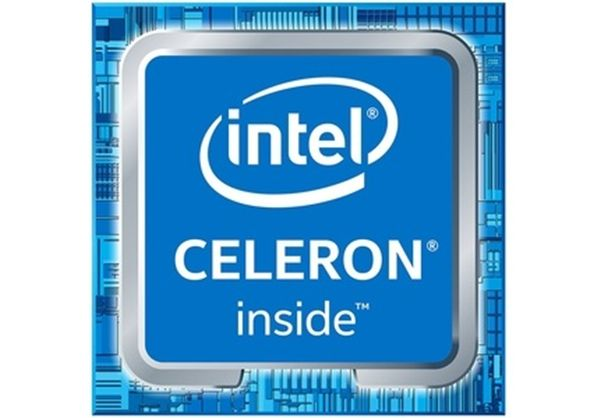
\includegraphics[width=0.3\textwidth]{figure/celeron.jpg}
    }
    \subfigure[Xeon]{
        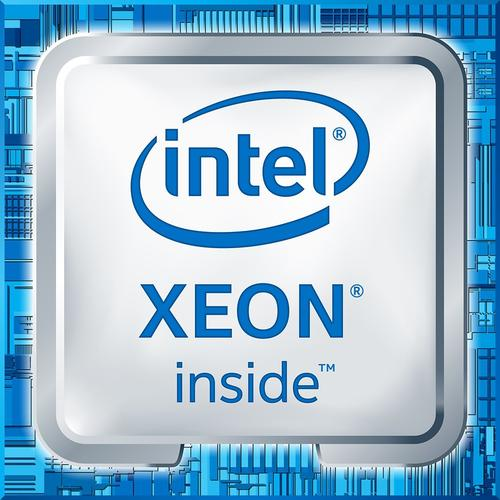
\includegraphics[width=0.21\textwidth]{figure/xeon.jpg}
    }
    \caption{Celeron和Xeon系列}
\end{figure}

\subsubsection{Pentium系列的后续产品}
世纪之交,Pentium系列产品的更新迭代还在继续。Intel相继推出了Pentium \uppercase\expandafter{\romannumeral3}(1999)、Pentium 4(2000)、Pentium M(2004)和Pentium D处理器。

其中,1999年推出的Pentium \uppercase\expandafter{\romannumeral3}处理器的主频首次突破1GHz。2002年,Intel在Pentium 4上首次运用了超线程技术。2005年,带有两个处理器内核的Pentium D推出,开启了CPU多内核的时代。以上三点是Pentium系列在这几年中主要的创新点。

然而在这一时期,从Pentium 4开始使用的P4架构“Netburst”出现了功耗和热量问题,在很长一段时间内,Intel无法将Netburst架构的处理器主频升至2GHz以上。随后,在此基础上改进的“Prescott”架构(被用于Pentium D)同样也出现了类似的问题。在一段短暂的时间中,Intel的在CPU领域的统治被AMD所打破。这也迫使Intel放弃Netburst架构,转而支持基于P6的Pentium M设计,这也促成了Intel新一代产品酷睿(Core)的诞生。

\subsection{2006-至今 酷睿(Core)的又一次辉煌}
随着AMD的步步紧逼,Intel不得不调整自己的策略。从2005年开始,Intel制定了一套“钟摆计划”(Tick-Tock),并在2006年推出了新一代酷睿(Core)产品,重新逆转了与AMD的竞争局面。


\section{AMD系列处理器发展历程}
\subsection{1969-1996 AMD公司的创立和Intel的代工厂}
\subsection{1996-1999 K5和K6:自研CPU的初尝试}
\subsection{1999-2006 K7到Athlon 64X2 AMD的崛起和辉煌}
\subsection{2006-2017 AMD失落的十年}
\subsection{2017-至今 锐龙(Ryzen)架构与AMD的重生}
%正文
\end{document}
